\documentclass[onecolumn, draftclsnofoot,10pt, compsoc]{IEEEtran}
\usepackage{graphicx}
\usepackage{url}
\usepackage{setspace}
\usepackage{listings}
\usepackage[center]{caption}
\usepackage{float}
\usepackage{pgfgantt}

\usepackage{geometry}
\geometry{textheight=9.5in, textwidth=7in}

% 1. Fill in these details
\def \CapstoneTeamName{The Cleverly Named Team}
\def \CapstoneTeamNumber{40}
\def \GroupMemberOne{Brian Hambleton}
\def \GroupMemberTwo{Dakota Alton}
\def \GroupMemberThree{Ian Band}
\def \GroupMemberFour{Ivan Halim}
\def \CapstoneProjectName{Converting Fortran to Python}
\def \CapstoneSponsorPerson{Genevieve Segol}

% 2. Uncomment the appropriate line below so that the document type works
\def \DocType{Design Document}
			
\newcommand{\NameSigPair}[1]{\par
\makebox[2.75in][r]{#1} \hfil 	\makebox[3.25in]{\makebox[2.25in]{\hrulefill} \hfill		\makebox[.75in]{\hrulefill}}
\par\vspace{-12pt} \textit{\tiny\noindent
\makebox[2.75in]{} \hfil		\makebox[3.25in]{\makebox[2.25in][r]{Signature} \hfill	\makebox[.75in][r]{Date}}}}
% 3. If the document is not to be signed, uncomment the RENEWcommand below
\renewcommand{\NameSigPair}[1]{#1}

%%%%%%%%%%%%%%%%%%%%%%%%%%%%%%%%%%%%%%%
\begin{document}
\begin{titlepage}
    \pagenumbering{gobble}
    \begin{singlespace}
        \hfill 
        \par\vspace{.2in}
        \centering
        \scshape{
            \huge CS Capstone \DocType \par
            {\large\today}\par
            \vspace{.5in}
            \textbf{\Huge\CapstoneProjectName}\par
            \vfill
            {\large Prepared for}\par
            {\Huge\NameSigPair{\CapstoneSponsorPerson}\par}
            {\large Prepared by }\par
            Group\CapstoneTeamNumber\par
            % 5. comment out the line below this one if you do not wish to name your team
            % \CapstoneTeamName\par 
            \vspace{5pt}
            {\Large
                \NameSigPair{\GroupMemberOne}\par
                \NameSigPair{\GroupMemberTwo}\par
                \NameSigPair{\GroupMemberThree}\par
                \NameSigPair{\GroupMemberFour}\par
            }
            \vspace{20pt}
        }
        \begin{abstract}  
        	This document describes the initial design choices for the development of a python based variably saturated flow and mass transport model. Design choices for user interface, development, and distribution are discussed herein. Specific design choices regard: 
        \end{abstract}     
    \end{singlespace}
\end{titlepage}
\newpage
\pagenumbering{arabic}
\tableofcontents
% 7. uncomment this (if applicable). Consider adding a page break.
%\listoffigures
%\listoftables
\clearpage

% 8. now you write!
\section{Introduction}
\subsection{Purpose}
This document serves as the outline for the application of research done by group40, with respect to the development of a python based variably saturated flow and mass transport model in two and three dimensions. 
\subsection{Scope}
The scope of this document is to identify each design and development component for our application, along with predicting how it will be done.  
\subsection{Time Line}
Below in fig. \ref{fig:my_label} the development time line for our application is outlined. In addition to what is below, every other week a test release of our application will be created and tested for quality assurance. House Keeping, in this context, refers to the initial set that must be done before development can be started. 
\begin{figure}[H]
    \centering
        \begin{ganttchart}[hgrid,vgrid]{1}{28}
            \gantttitle{Capstone Group40 Development Time Line}{28} \\
            \gantttitle{Week}{28}\\
            \gantttitlelist{1,...,28}{1} \\
            \ganttgroup{House Keeping}{1}{4} \\
            \ganttbar{Transcribe Fortran}{1}{2} \\
            \ganttbar{Setup github repo}{1}{2}\\
            \ganttbar{Setup python tooling}{2}{2}\\
            \ganttgroup{Development}{5}{16} \\
            \ganttbar{Translate Fortran}{5}{7} \\
            \ganttbar{Develop GUI}{5}{8} \\
            \ganttbar{Develop Mesh Builder}{5}{8} \\
            \ganttbar{Merge GUI and Mesh Builder}{9}{12}\\
            \ganttbar{Strech Goals}{13}{16}\\
            \ganttgroup{Presentation}{17}{28}\\
            \ganttbar{1.0 Release}{17}{18}\\
            \ganttbar{V1.0 QA Testing}{19}{23}\\
            \ganttbar{Expo}{24}{24}\\
            \ganttbar{Final Report}{25}{28}
        \end{ganttchart}
    \caption{Gantt chart representing development time line from the first week in December to June 15}
    \label{fig:my_label}
\end{figure}{}


\subsection{Summary}
Our application is meant to replace a legacy fortran version of the variably saturated flow and mass transport model. It will do this by converting the legacy code base to python and building a graphical user inter faces on top of it to better facilitate ease of use. Accomplishing these tasks will allow for two goals to be met. First, converting to python means that the application will be able to run on a wider array of devices. Second, adding a GUI to the application will improve user experience by making data input and output cleaner.
\subsection{Revision History}
\section{References}

\section{Glossary}

\begin{itemize}
    \item \textit{freezing} - In the context of Python, "freezing" refers to bundling a program's dependencies along with a python interpreter into an executable file. 
    \item \textit{pip} - This is a Python tool used for installing external python libraries. 
    \item \textit{requirements.txt} - This is a file that hold information on what external libraries are being consumed by our application. 
\end{itemize}{}

\section{Component Overview}
Fig. \ref{fig:comp-own} states who is, at a high level, responsible for which component. Transcribing and translating will be done by all of group40. The 3D Approximations component represents a stretch goal as such the owner will be assigned at a point in time when it is clear if the goal can be met. \\\\
\begin{figure}[H]
    \centering
    \begin{tabular}{|c|c|}
        \hline
         Component & Owner \\\hline
         Code Transcribing & Ian Band \\\hline
         Code Translation & Ian Band \\\hline
         Code Reuse & Ian Band \\\hline
         3D Approximations & N\textbackslash A \\\hline
         Environment Manager & Dakota Alton \\\hline
         Distribution & Dakota Alton \\\hline
         Automation & Dakota Alton \\\hline
         Finite Element Mesh Generator & Ivan Halim \\\hline
         File Format & Ivan Halim \\\hline
         3-Dimensional Mesh Plotter & Ivan Halim \\\hline
         PyQT GUI & Brian Hambleton \\\hline
         CLI & Brian Hambleton \\\hline
    \end{tabular}{}
    \caption{Components and associated owner}
    \label{fig:comp-own}
\end{figure}{}

\section{Simulation}
\subsection{Transcribing}
The Fortran code provided by the client must be transcribed into text files that can be compiled.
\subsubsection{Context}
Source code was provided to our team in the form of a scanned PDF document. In order to use this code, it must be manually transcribed by our team into text files. Each subroutine in the source code will be transcribed in its own text file to make reuse of that routine more convenient. Manually transcribing the code will give our team familiarity with the codes functionality. 
\subsubsection{Set Up}
Each team member will be assigned a number of subroutines to transcribe. 

\subsection{Code Translation}
Functioning simulation code provided by the client will be translated from Fortran to Python 3. 
\subsubsection{Context}
The simulation wrapper and interfaces between the simulation, data input, data output, and data visualization will all be written in Python 3. 
\subsubsection{Set Up}
Developers will directly translate the main routine of each simulation. This mainly consists of calling the right Fortran subroutines from Python in the right order, and correctly passing arguments to each subroutine. 


\subsection{Code Reuse}
\subsubsection{Context}
It is possible to reuse a large portion of the Fortran code base along side code written in Python. Doing so introduces design trade offs which are not discussed in depth in this section. In essence, reusing Fortran code alongside Python ensures an accurate, high performance, and easy to develop simulation will be produced. Time saved in this part of development allows for more time and resources to be spent on other parts of the project where code reuse is not an option. 
\subsubsection{Set Up}
Developers on our team will use the F2PY library to create a signature file from the Fortran source that is usable within Python code. Developers will create signature files by running:
\begin{lstlisting}[language=bash]
  $ python -m numpy.f2py -c <Fortran source file> -m <package name>
\end{lstlisting}


\subsection{2D and 3D Approximations}
\subsubsection{Context}
The original code base consists of two related, but independent simulation tools. Our team will aim to recreate the 2D simulation before moving onto the 3D simulation as a stretch goal. In this way, we can use what we learn from creating the 2D simulation to help us with the 3D simulation. 


\section{Development \& Deployment}
\subsection{Environment Manager}

For this project we will be using the tool virtualenv to manage our applications external packages.

\subsubsection{Context}
The main point of having an environment manager is to be able to develop on any computer while maintaining a consistent set of external libraries. This is a necessary component of our design for we will be developing on different operating systems. Just as well, our freezing tool of choice is meant to run on the operating system that our application will run on, so keeping a consistent environment will mitigate any issues concerning building on any operating system. 
\subsubsection{Set Up}

Setting up virtualenv is something that each developer will have to do. They will set virtualenv up by cloning the source repository and running the following command at the root of the repository:
\begin{lstlisting}[language=bash]
  $ python3 -m venv env
\end{lstlisting}
\noindent
This will create a directory called "env" that represents a virtual environment for managing python. At this point the workflow outlined in the following section must be adhered to. \\\\
\noindent
Note that the directory created should not be placed into source control.

\subsubsection{Workflow}
\begin{enumerate}
    \item enable the virtual environment with: 
    \begin{lstlisting}[language=bash]
      $ source env/bin/activate
    \end{lstlisting}

    \item program and install packages as one normally would.
    
    \item deactivate the virtual environment with: 
     \begin{lstlisting}[language=bash]
      $ deactivate
    \end{lstlisting}
\end{enumerate}{}
\noindent
Note that when a package is installed with pip, one musts run \textit{\$ pip freeze $>$ requirements.txt}, to make sure that the library is known in source control.

\subsection{Distribution}

To build an executable of our application, we have chosen to use the tool PyInstaller.

\subsubsection{Context}
Utility of an application is predicated on the ability to run the application. Instead of requiring users to install a python interpreter to run our application, it  would be more convenient to download an executable version of our code. To do this, our code base must be "frozen" that is, all dependencies must be bundled into a sole executable file. Furthermore, our code must be usable on Windows and Mac so configuring PyInstaller to build an executable must be done to allow building Windows and Mac. 
\subsubsection{Set Up}

PyInstaller is a package that can be installed with pip. It will be added to the projects requirements.txt just after setting up the git hub repository. PyInstaller can then be run on the main file of our application to build an executable.
\\\\
\noindent
For actually distributing our application we will tag branches in git for our current release version and add the appropriate executable files there. 
\subsection{Automation}

To automate the testing our application we will be using the continuous integration (CI) service provided by TravisCI.

\subsubsection{Context}

Group development is best done when there is an identifiable standard to meet. Requiring that each developer run tests on their local machines is fickle; one's system, despite preventative measures, can be slightly different from another person's system leading to a false sense of quality. This is the primary case for using an independent CI service.    

\subsubsection{Set Up}
 
 TravisCI is will be set up by linking our git hub repository to our TravisCI account. Then we just add a travis.yml that specifies our version of python and which commands that must be run for our tests to run. An example travis.yml file would be:
 
 \begin{figure}[H]
     \centering
	 \begin{lstlisting}
            language: python
            python:
              - "3.3"
            install:
              - pip install -r requirements.txt
            script: pytest
        \end{lstlisting}
     \caption{Example travis.yml file}
     \label{fig:travis-ci}
 \end{figure}{}



\section{Visualization}
\subsection{Finite Element Mesh Generator}
To generate our mesh, we have chosen PyVista.
\subsubsection{Context}
A mesh generator is a very important component to any finite element solver. The purpose of a mesh generator is to create complex geometries and then discretize it into small simple shapes, such as triangles or quadrilaterals. The purpose of the discretization is to allow us to perform finite element analysis on complicated shapes, because we know how to perform calculations on a triangle but not directly on complicated spaces and shapes such as a roadway bridge.
\subsubsection{Dependencies}
The following modules are the required dependencies of PyVista:
\begin{itemize}
    \item vtk - PyVista is built on top of the VTK library
    \item numpy - Provides direct data access for meshes
    \item imageio - Used for saving screenshots
    \item appdirs - Data management for example datasets.
\end{itemize}
\subsubsection{Set Up}
To install PyVista simply type on the command line,
\begin{lstlisting}[language=bash]
  $ pip install pyvista
\end{lstlisting}
\subsubsection{Mesh Generation}
A mesh is a geometrical representation of a 2D surface or 3D volume. A mesh consists of \textbf{nodes}, \textbf{edges} and \textbf{elements}.
\begin{itemize}
    \item \textbf{Node:} The XYZ coordinates of the underlying structure
    \item \textbf{Edge:} The connectivity between nodes
    \item \textbf{Element:} The area or volume bounded by the edges.
\end{itemize}

\begin{figure}[H]
\centering
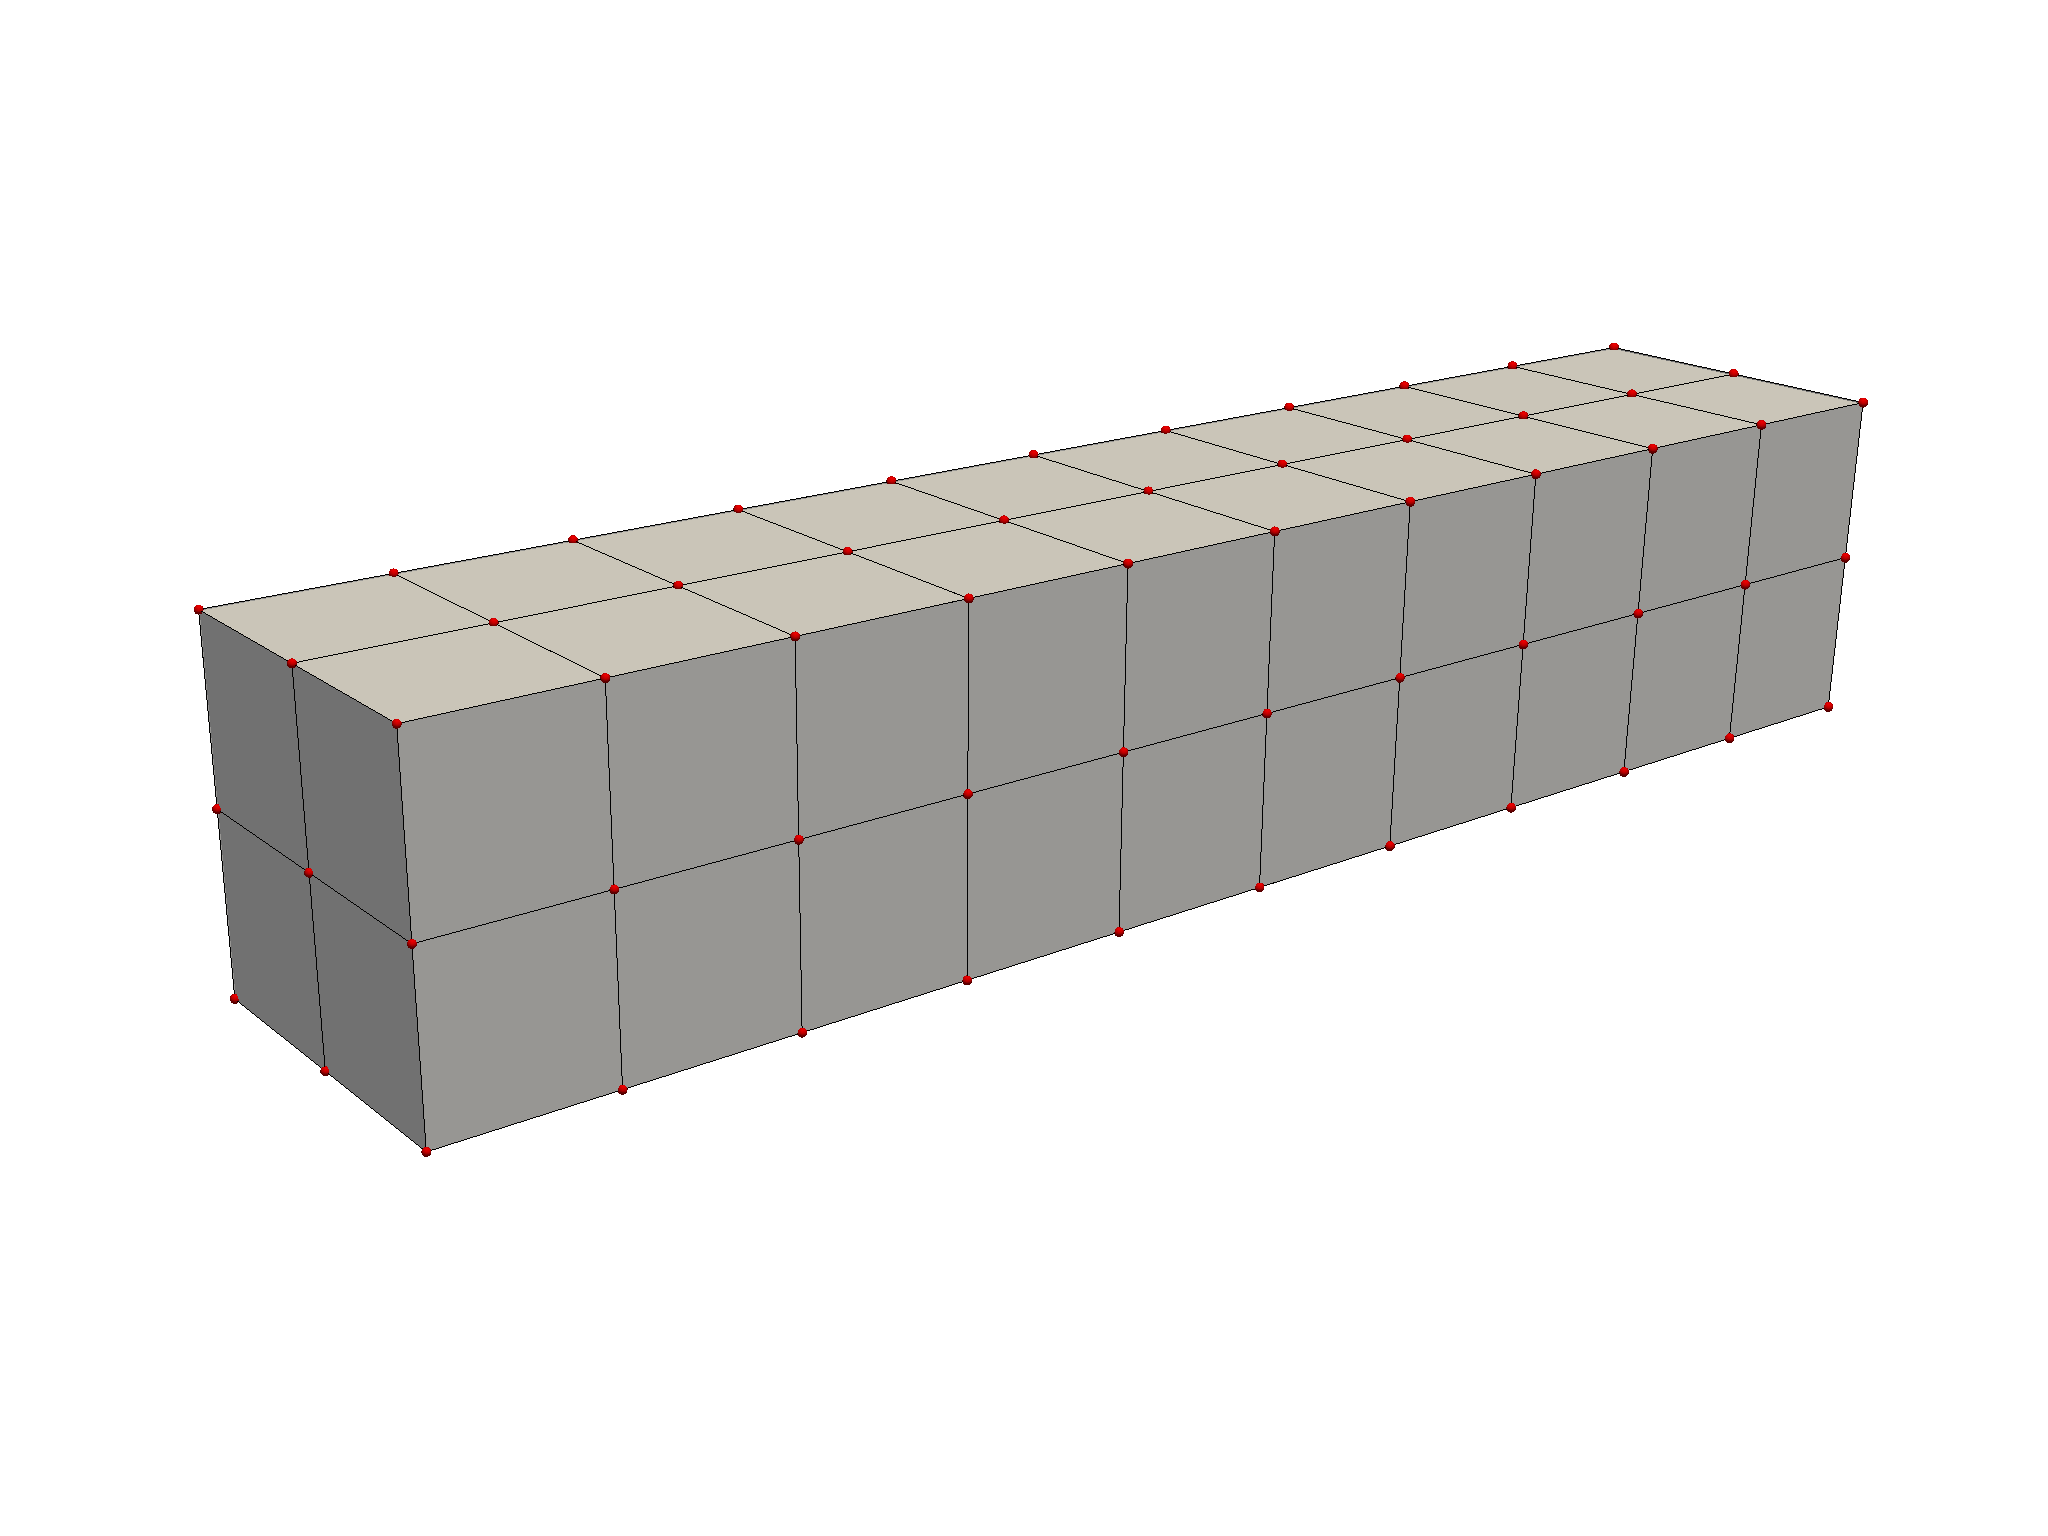
\includegraphics[scale=0.2]{mesh.png}
\caption{An example mesh.}
\label{fig:mesh}
\end{figure}

\noindent
To create a mesh in PyVista, we will be using the PolyData object. The PolyData object accepts NumPy arrays of vertices and faces. The vertex array contains the XYZ coordinates of each point in the mesh and the face array contains the number of points of each face and the indices of the vertices which comprise that face.

\begin{lstlisting}[language=python]
    # mesh points
    vertices = np.array([[0, 0, 0],
                         [1, 0, 0],
                         [1, 1, 0],
                         [0, 1, 0],
                         [0.5, 0.5, -1]])

    # mesh faces
    faces = np.hstack([[4, 0, 1, 2, 3],  # square
                       [3, 0, 1, 4],     # triangle
                       [3, 1, 2, 4]])    # triangle

    mesh = pv.PolyData(vertices, faces)
\end{lstlisting}

\subsection{File Format}
For the representation of mesh, we have chosen the VTK XML file format.
\subsubsection{Context}
Before we visualize our mesh, we have to make sure that the data produced by the mesh generator is in a file format that the plotter can accept. Not all file formats are created equal. Some formats are more space-efficient or support more features such as parallel reading and rendering for large datasets. For this reason, we have chosen the VTK XML file format due to its flexibility.
\subsubsection{Dataset Types}
VTK can handle several kinds of datasets, for points data and cells data. The primary are:
\begin{itemize}
    \item \textbf{ImageData:} Regularly spaced points data.
    \item \textbf{RectilinearGrid:} Regularly spaced points data but spacing can be not uniform.
    \item \textbf{StructuredGrid:} Not regular and not uniform points of data.
    \item \textbf{UnstructuredGrid:} Not regular and not uniform points data, but can handle all cell types.
    \item \textbf{PolyData:} Can be used for any polygonal data.
\end{itemize}

\subsubsection{General Structure}
The general structure for each dataset format is as follows:\\

\noindent
\textbf{ImageData:} For ImageData you only have to set the mesh dimensions (nx, ny, nz), mesh origin (x0, y0, z0) and cell dimensions (dx, dy, dz). Thus, points data are regularly and uniformly spaced.

\begin{figure}[H]
\centering
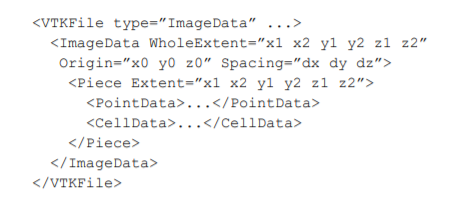
\includegraphics{ImageData.png}
\caption{ImageData format.}
\label{fig:imagedata}
\end{figure}

\noindent
\textbf{RectilinearGrid:} In RectilinearGrid, you have to specify the nodes coordinates along the three axes, Ox, Oy, Oz.

\begin{figure}[H]
\centering
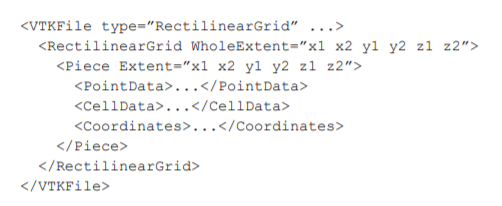
\includegraphics{RectilinearGrid.png}
\caption{RectilinearGrid format.}
\label{fig:rectilineargrid}
\end{figure}

\noindent
\textbf{StructuredGrid:} For StructuredGrid, you have to specify the coordinates for all mesh nodes.

\begin{figure}[H]
\centering
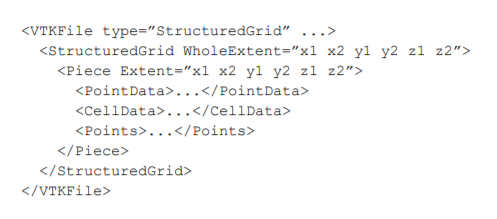
\includegraphics{StructuredGrid.png}
\caption{StructuredGrid format.}
\label{fig:structuredgrid}
\end{figure}

\noindent
\textbf{UnstructuredGrid:} Each UnstructuredGrid piece specifies a set of points and cells independently from the other pieces. The points are described explicitly by the Points element. The cells are described explicitly by the Cells element.

\begin{figure}[H]
\centering
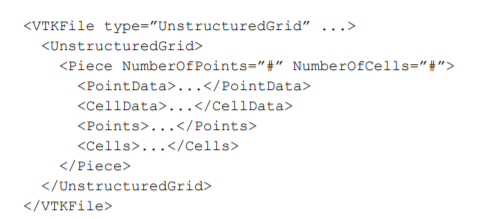
\includegraphics{UnstructuredGrid.png}
\caption{UnstructuredGrid format.}
\label{fig:unstructuredgrid}
\end{figure}

\noindent
\textbf{PolyData:} Each PolyData piece specifies a set of points and cells independently from the other pieces. The points are described explicitly by the Points element. The cells are described explicitly by the Verts, Lines, Strips, and Polys elements.

\begin{figure}[H]
\centering
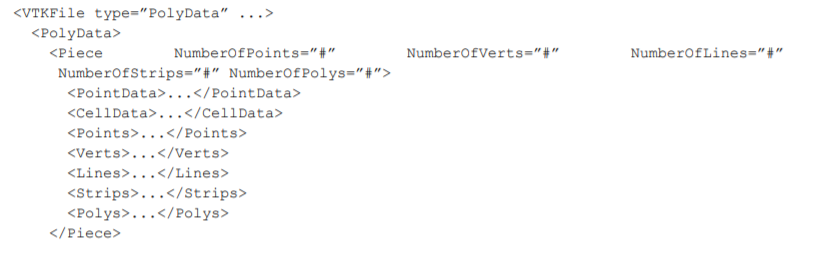
\includegraphics[scale=0.8]{PolyData.png}
\caption{PolyData format.}
\label{fig:polydata}
\end{figure}

\subsubsection{File Conversion}
Rather than writing our mesh file from scratch, it is better to generate our mesh from one of the mesher programs and convert the output into our desired file format. To do this, we will be using a Python module called \textbf{Meshio}.\\

\noindent
Meshio is a Python library that provides interoperability between all the various mesh formats. Meshio can read and write all of the mesh formats mentioned above and smoothly converts between them.\\

\noindent
To convert a file, simply call,
\begin{lstlisting}[language=bash]
     $ meshio-convert input.msh output.vtu
\end{lstlisting}

\noindent
In Python, simply do,
\begin{lstlisting}[language=python]
     import meshio

     mesh = meshio.read(filename)
     meshio.write("foo.vtk", mesh)
\end{lstlisting}


\subsection{3-Dimensional Mesh Plotter}
For this project, we have chosen PyVista as our visualization library.
\subsubsection{Context}
After generating our mesh, we want to be able to visualize it so we can see directly the results of our analysis. PyVista supports many plotting functions that are highly controllable and Pythonic.
\subsubsection{Dependencies}
The following modules are the required dependencies of PyVista:
\begin{itemize}
    \item vtk - PyVista is built on top of the VTK library
    \item numpy - Provides direct data access for meshes
    \item imageio - Used for saving screenshots
    \item appdirs - Data management for example datasets.
\end{itemize}
\subsubsection{Set Up}
To install PyVista simply type on the command line,
\begin{lstlisting}[language=bash]
  $ pip install pyvista
\end{lstlisting}
\subsubsection{Plotting}
To plot an object, simply call the \textbf{pyvista.plot} function that is binded to each PyVista data object.

\begin{lstlisting}[language=python]
    mesh = pv.PolyData(vertices, faces)
    mesh.plot()
\end{lstlisting}

\noindent
To better customize your plot, you can also create a \textbf{pyvista.plotter}

\begin{lstlisting}[language=python]
    plotter = pv.Plotter()
    plotter.add_mesh(mesh)
    cpos = plotter.show() 
\end{lstlisting}

\noindent
To display interactive plots, we can also use the \textbf{pyvista.BackgroundPlotter} to create a rendering window in the background that remains interactive while the user performs their processing. This creates the ability to update the plotter in real-time.

\begin{figure}[H]
\centering
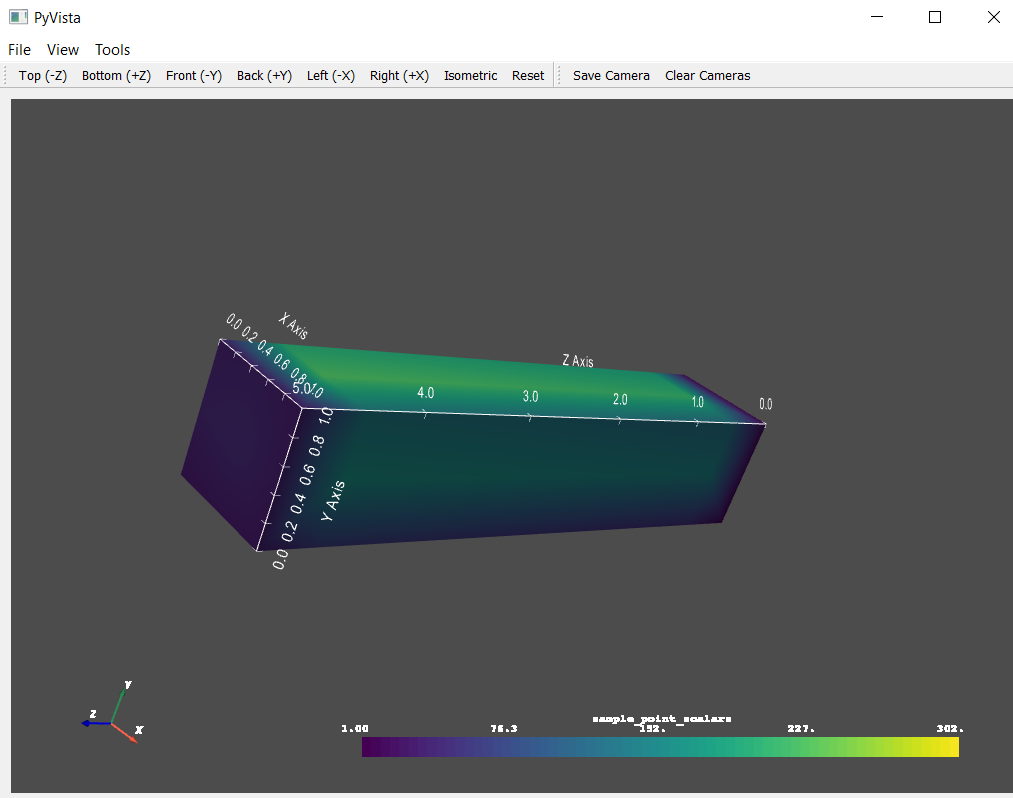
\includegraphics[scale=0.5]{backgroundplotter.png}
\caption{A rendering window that runs in the background, allowing you to update the data in real-time.}
\label{fig:backgroundplotter}
\end{figure}

\section{User Interface}
The user interface represents the frontend of the system which allows users to setup, run, and review simulations. The two ways for users to perform these three tasks will be through the graphical user interface and a command line interface. Both interfaces will allow users to input the numerous parameters required to run a simulation. These can be supplied via the GUI’s input forms or by submitting a file path to a file containing appropriately formatted data.
\subsection{PyQT GUI}
\subsubsection{Context}
The GUI will be constructed using the Python bindings of the QT framework, PyQT. This includes substantial classes, e.g. QApplication, QWidget and QInputDialog, and methods to generate all the necessary parts of the GUI. PyQT was chosen over the numerous other Python libraries for constructing GUIs because of its widespread use in modern software applications, seamless interaction with other libraries being used (PyVista, NumPy, etc.), and availability of training documentation.
\subsubsection{Install}
 Before PyQT5 can be used to implement the GUI it must first be downloaded and installed. After downloading use the command:
\begin{lstlisting}[language=python]
    pip install PyQt5
\end{lstlisting}
The base object used by PyQT is the QApplication object. The base class for all objects included in the GUI is QWidget. As the name suggests, QInputDialog contains methods for including various input containers in the GUI. These QT classes are the main sources of objects that will be used within the programs GUI.

\subsubsection{Composition}
The GUI must first provide a way for the user to build their mesh before any calculations can be performed. The mesh is constructed of nodes described by x, y, and z coordinates for the 3D model, x and y for the 2D model. Individual nodes also have attributes to define their material and state. Groups of nodes represent an element which also have attributes to define their state. The GUI will allow the user to supply these sets of attributes through numerical input or via a formatted file. Figure 11 shows an application window with navigation buttons to accomplish these tasks via manual input through the navigation buttons and input fields, or the ability to provide the information in a pre-formatted file. Figure 13 shows an example of a way for a user to provide their nodal information. Each individual cell below the header row is an input field where numerical values can be entered to supply the attributes of each node. Figure 14 contains similar input for each element in the mesh.\\
After building the mesh the user will have the ability to tweak the attributes of each node, face and model variables before running the model. Figure 15 shows an example of a screen with these capabilities.
\begin{figure}[H]
\centering
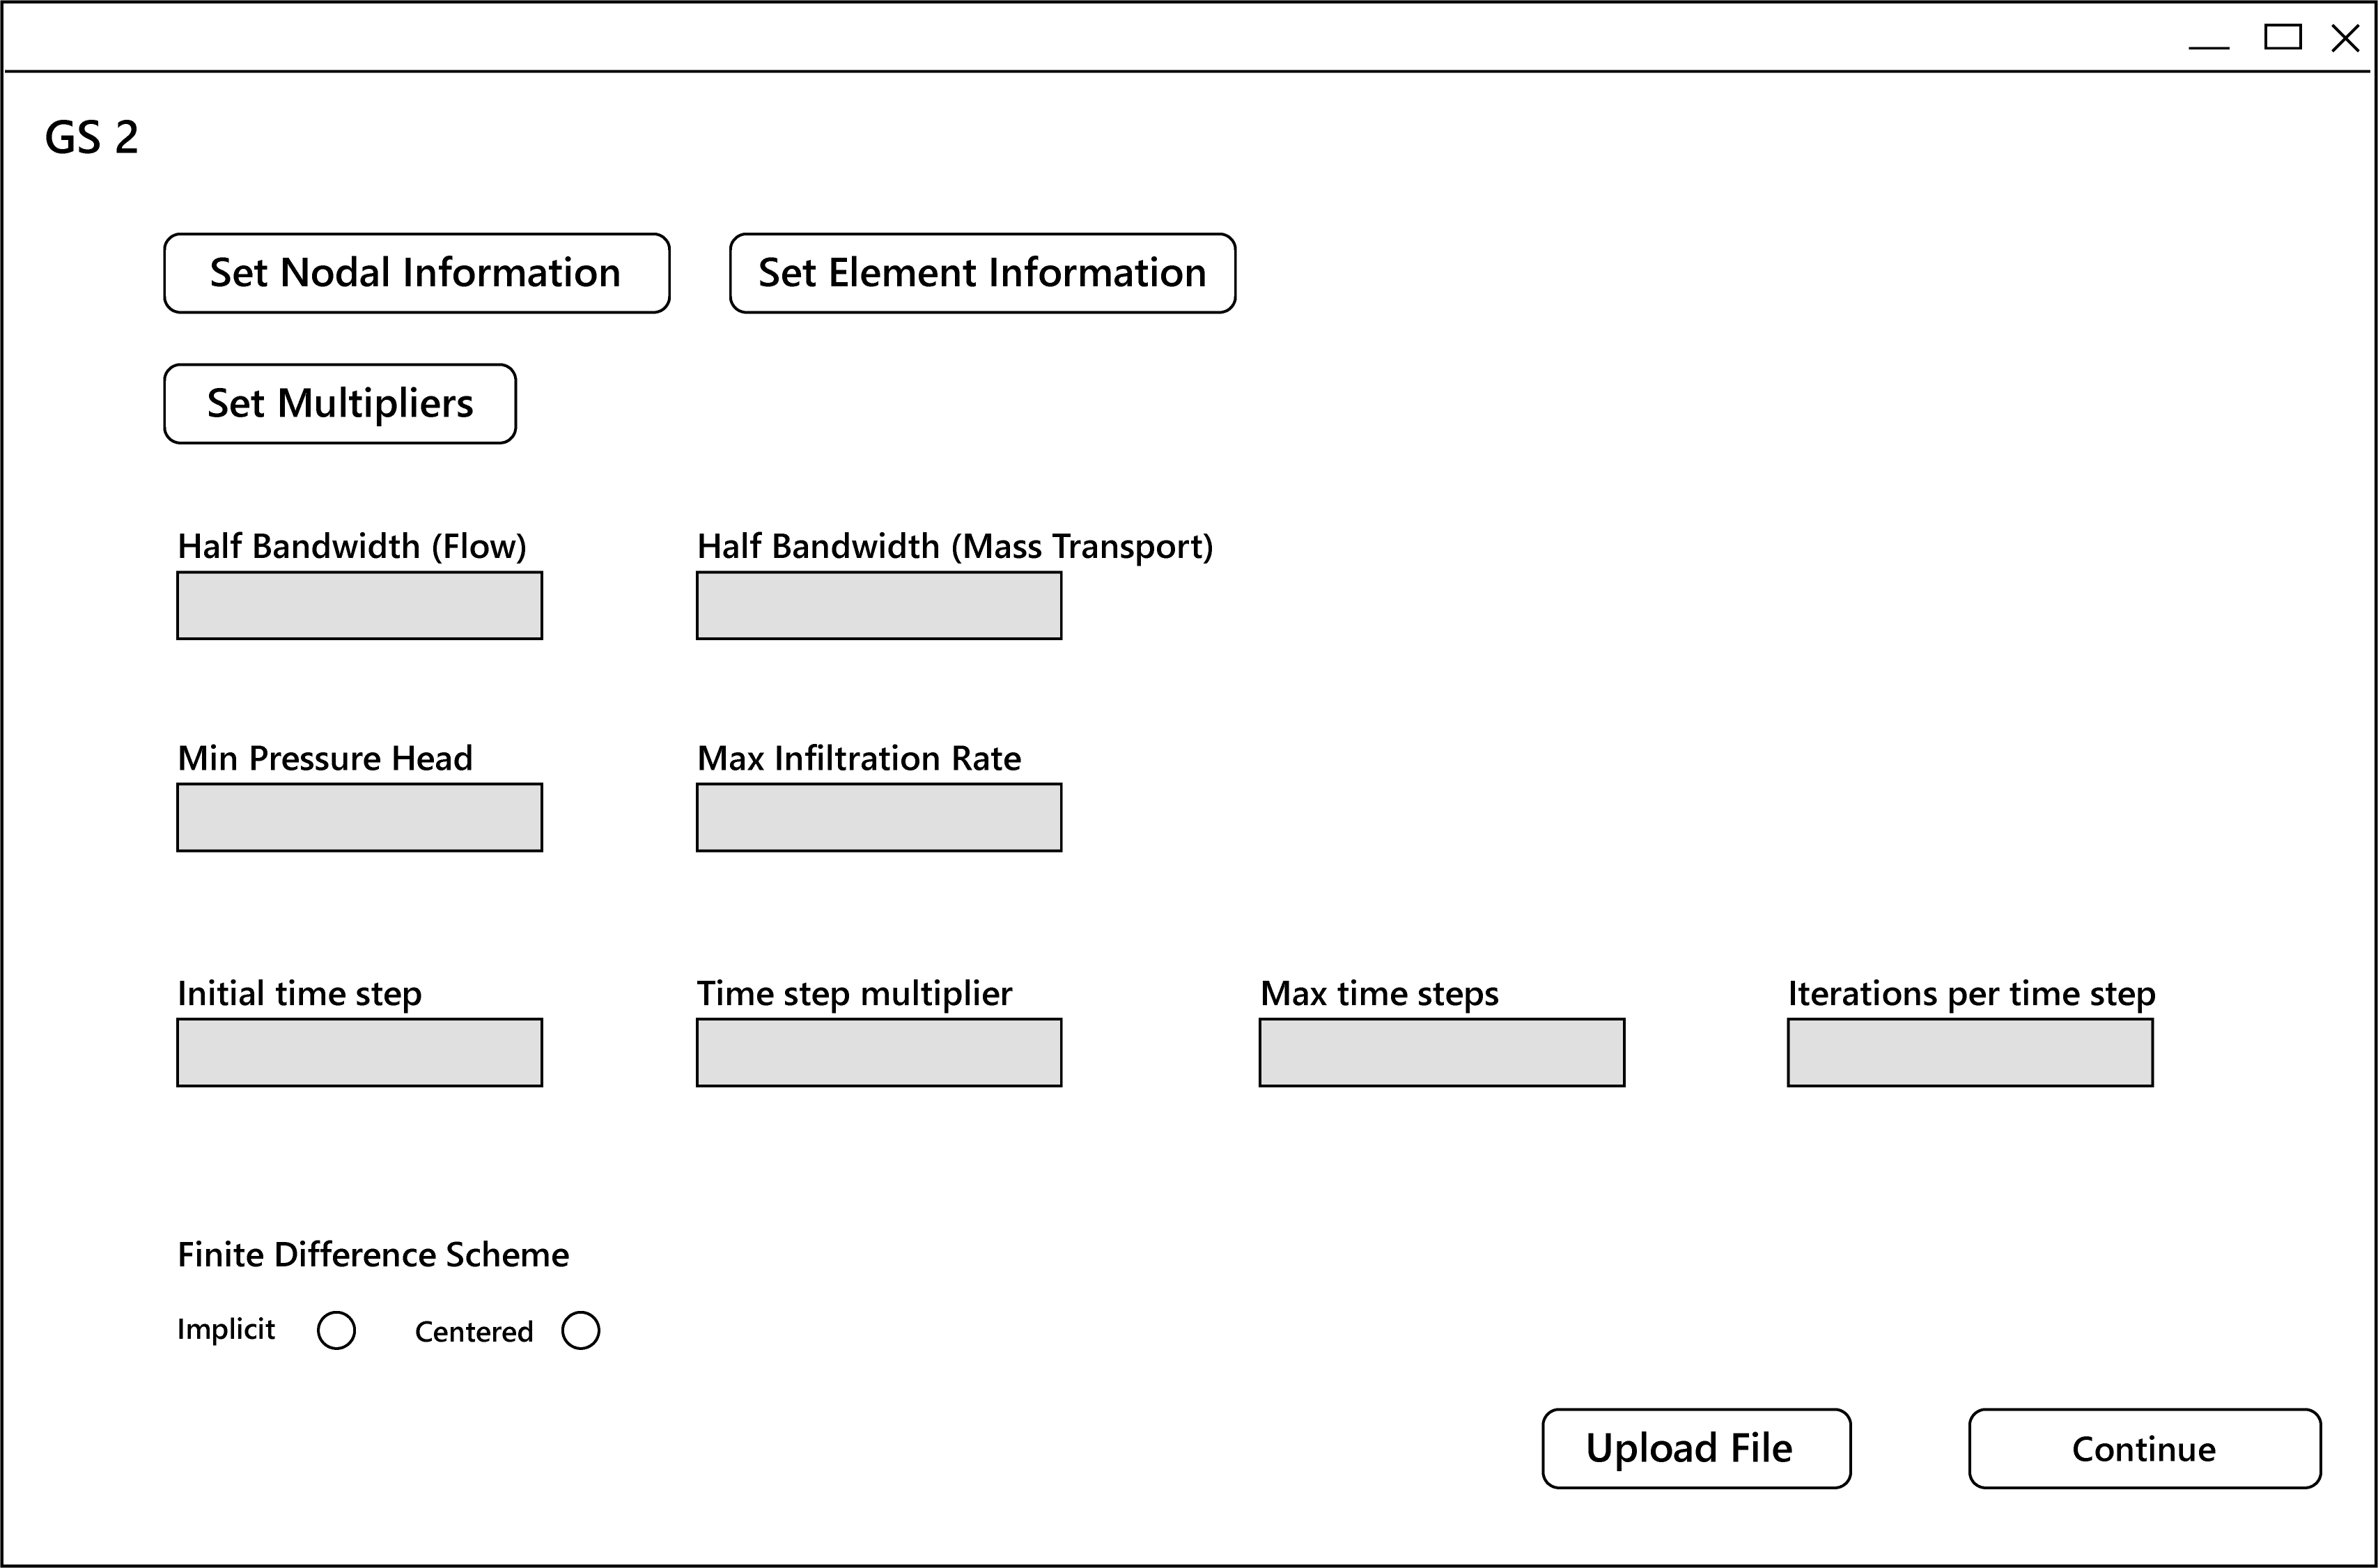
\includegraphics[scale=0.5]{GS2_home.png}
\caption{Project Main Screen}
\label{fig:Project Screen}
\end{figure}

\begin{figure}[H]
\centering
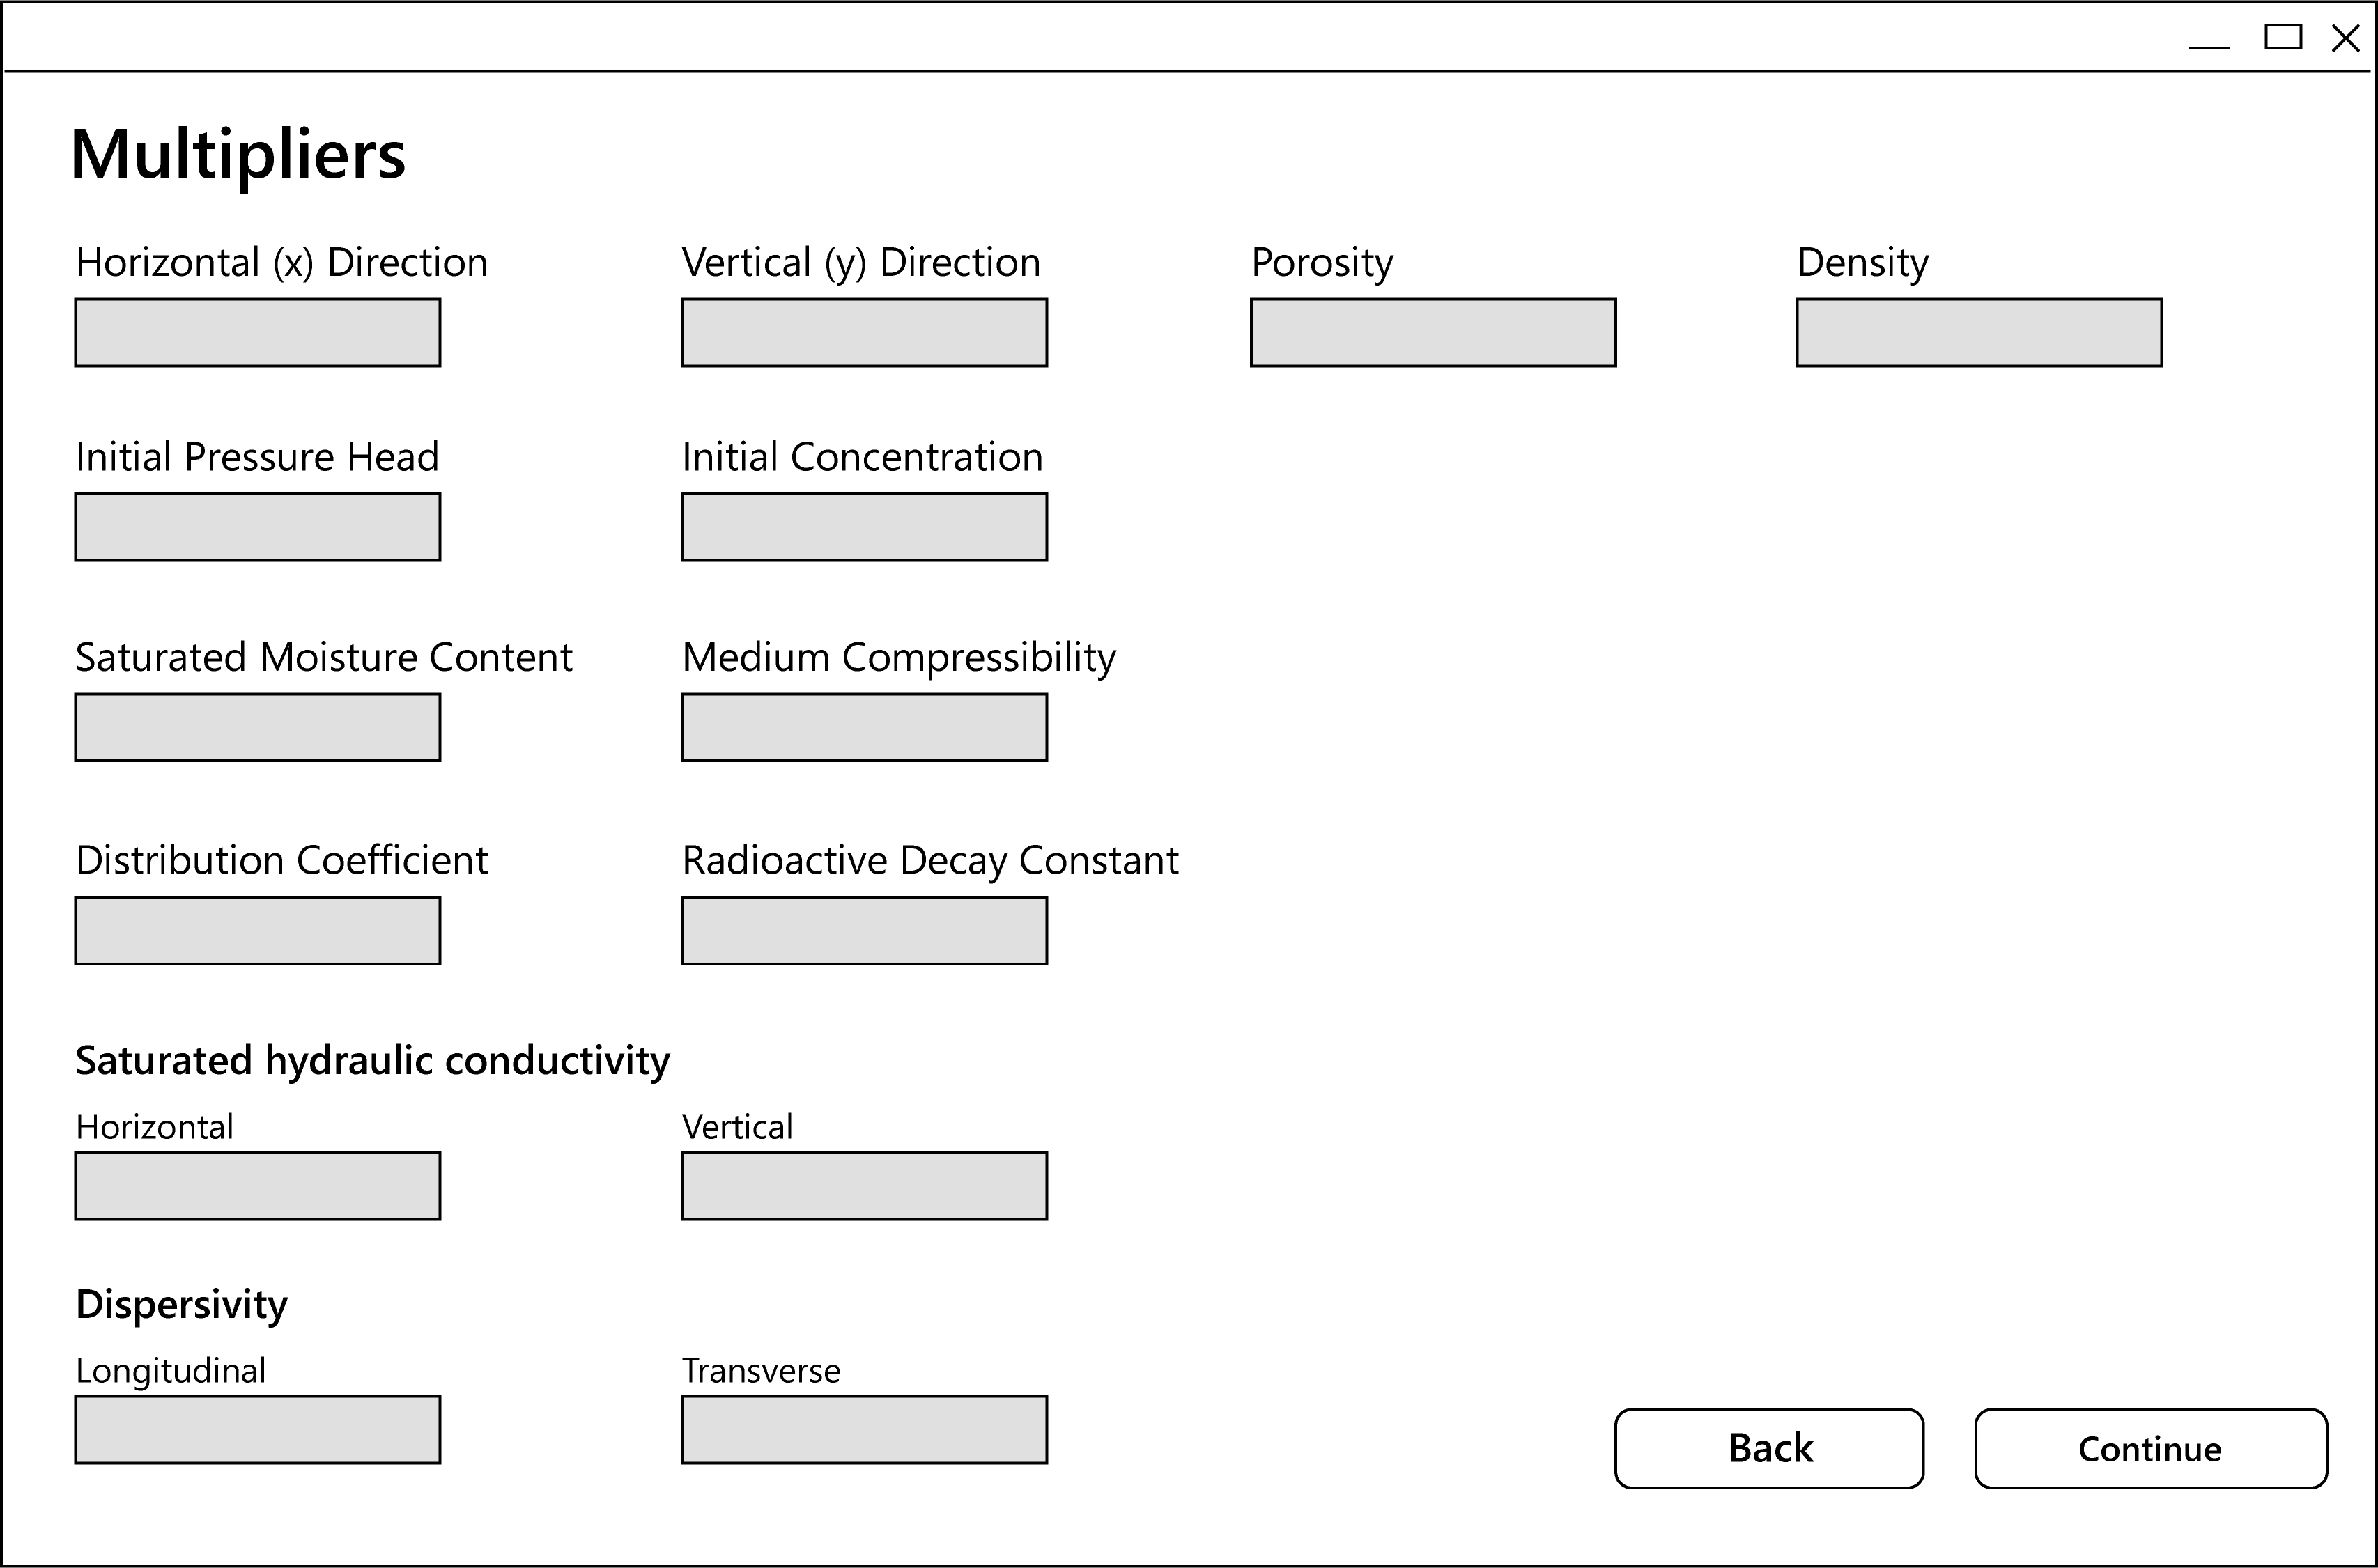
\includegraphics[scale=0.5]{GS2_multipliers.png}
\caption{Screen to initialize variable multipliers}
\label{fig:Multiplier Screen}
\end{figure}

\begin{figure}[H]
\centering
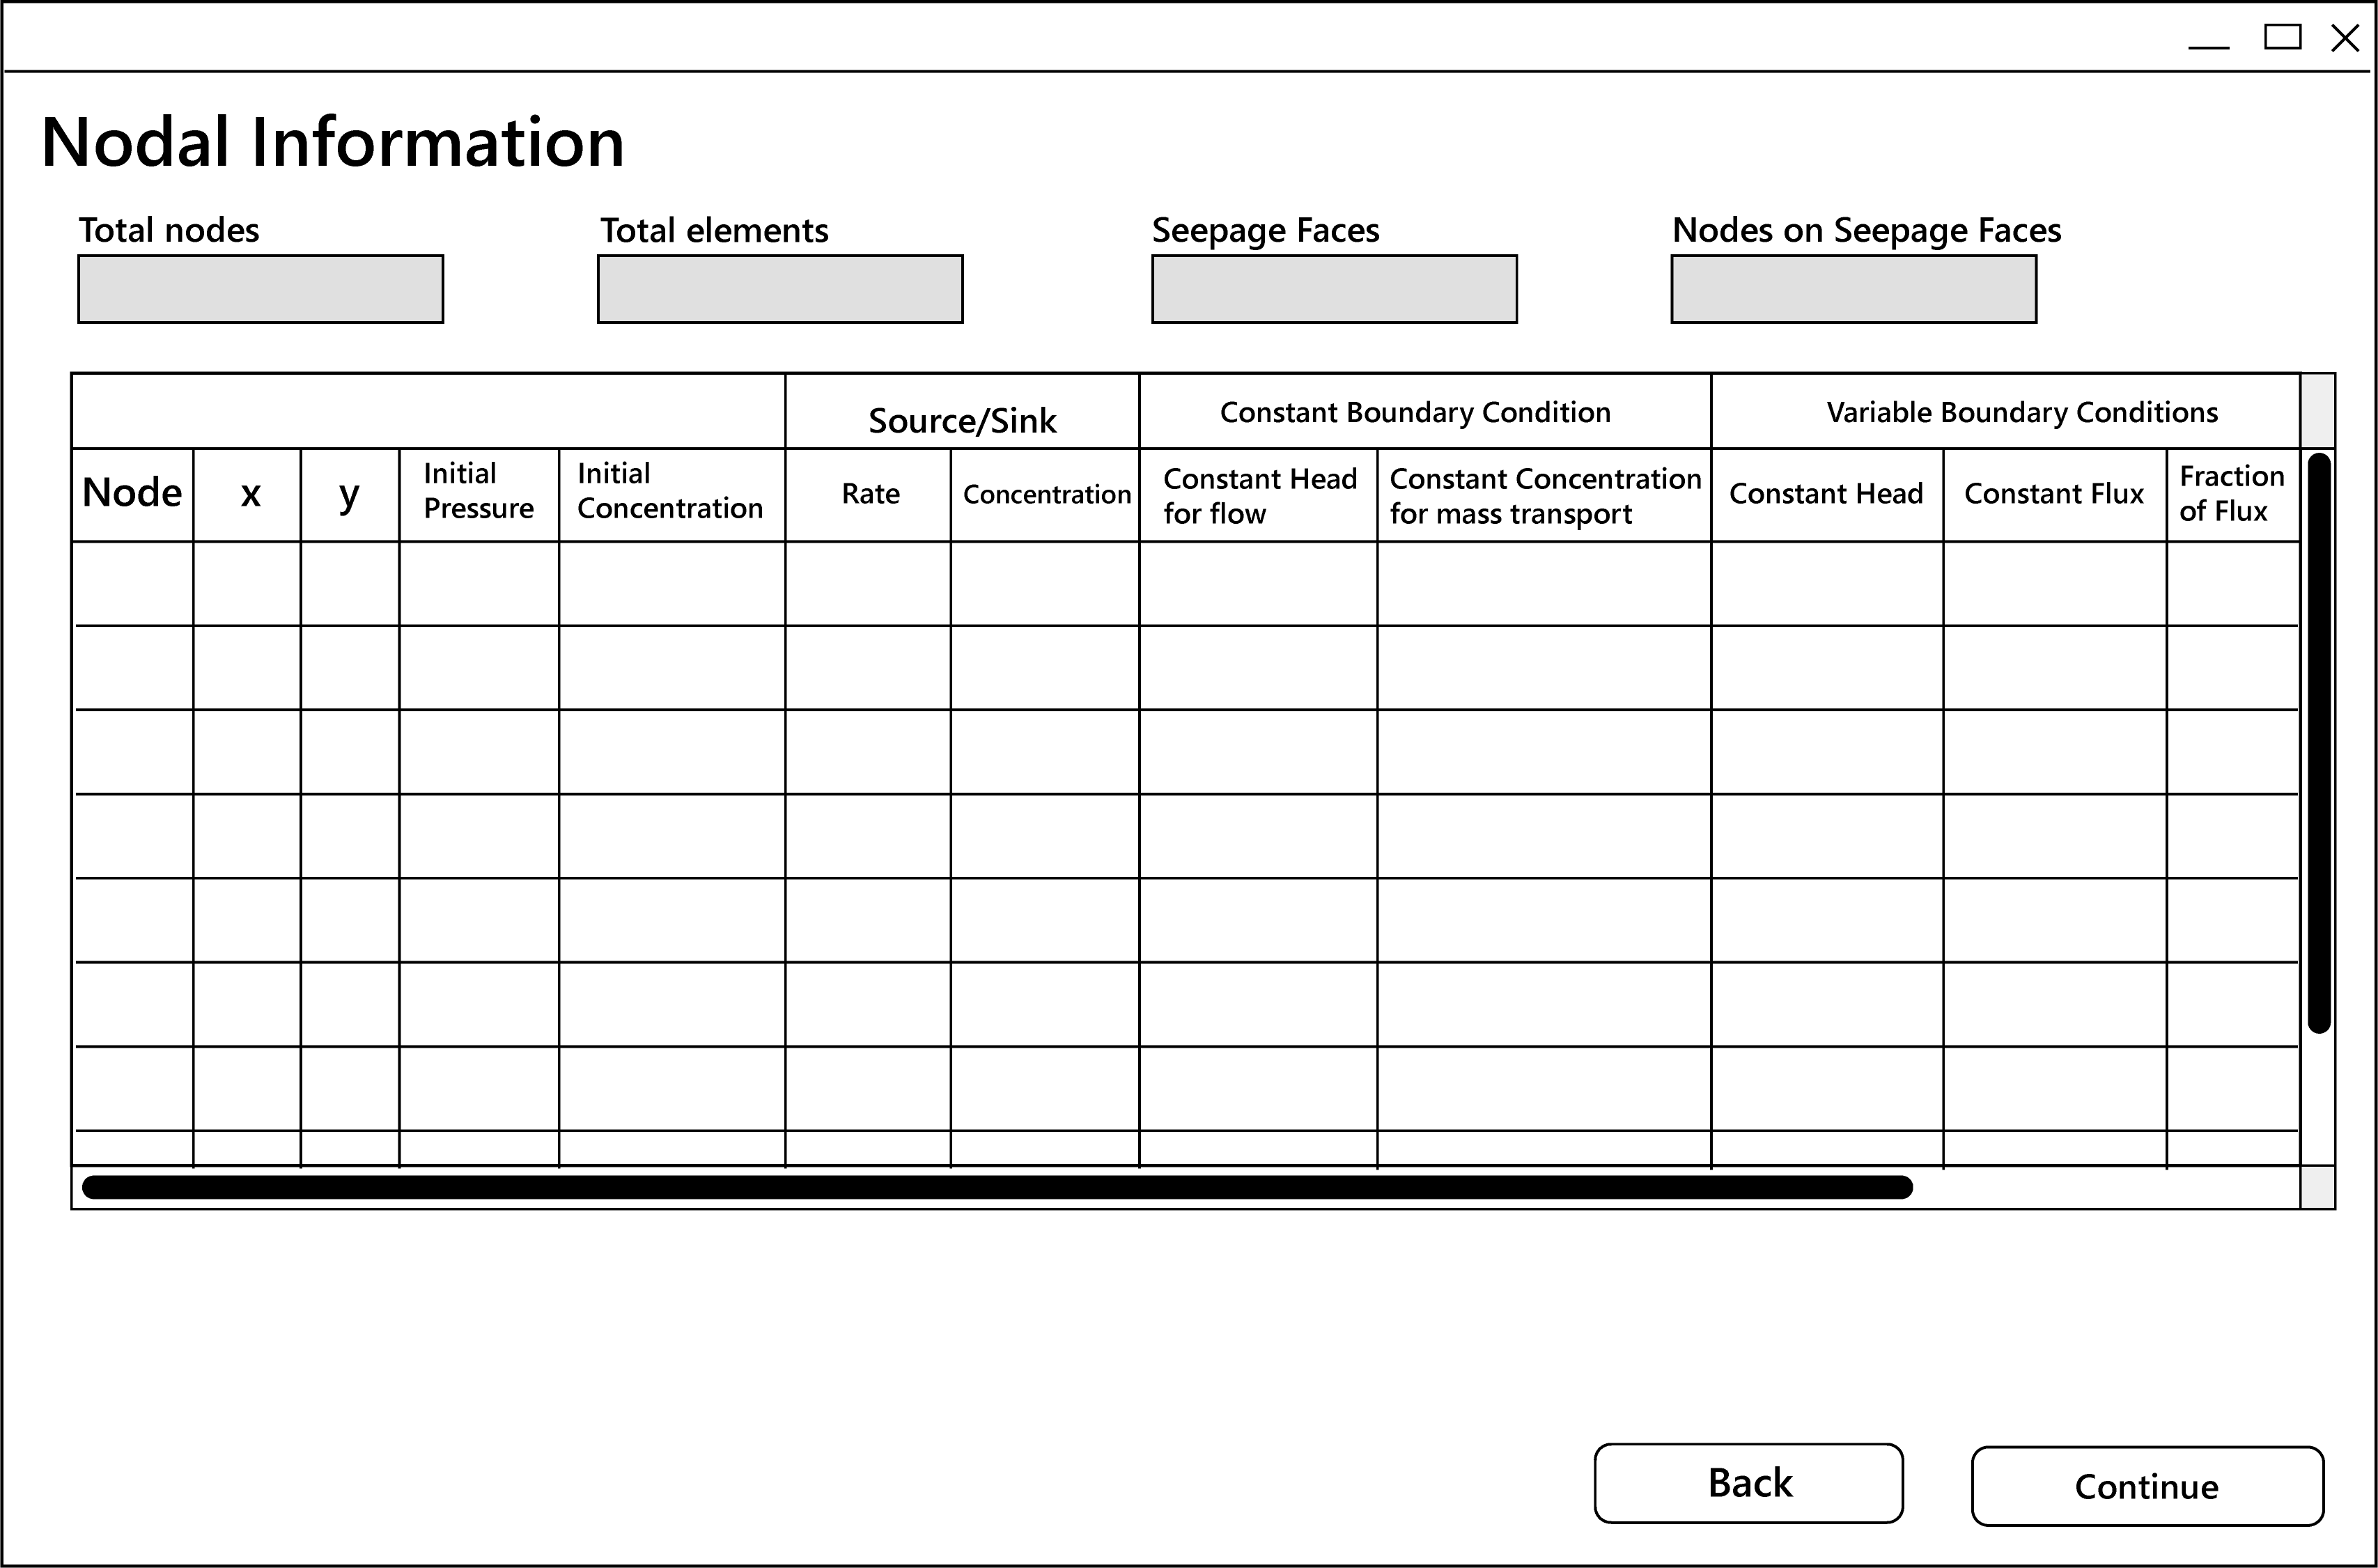
\includegraphics[scale=0.5]{GS2_nodal.png}
\caption{Screen to set nodal data}
\label{fig:Nodal Information Screen}
\end{figure}

\begin{figure}[H]
\centering
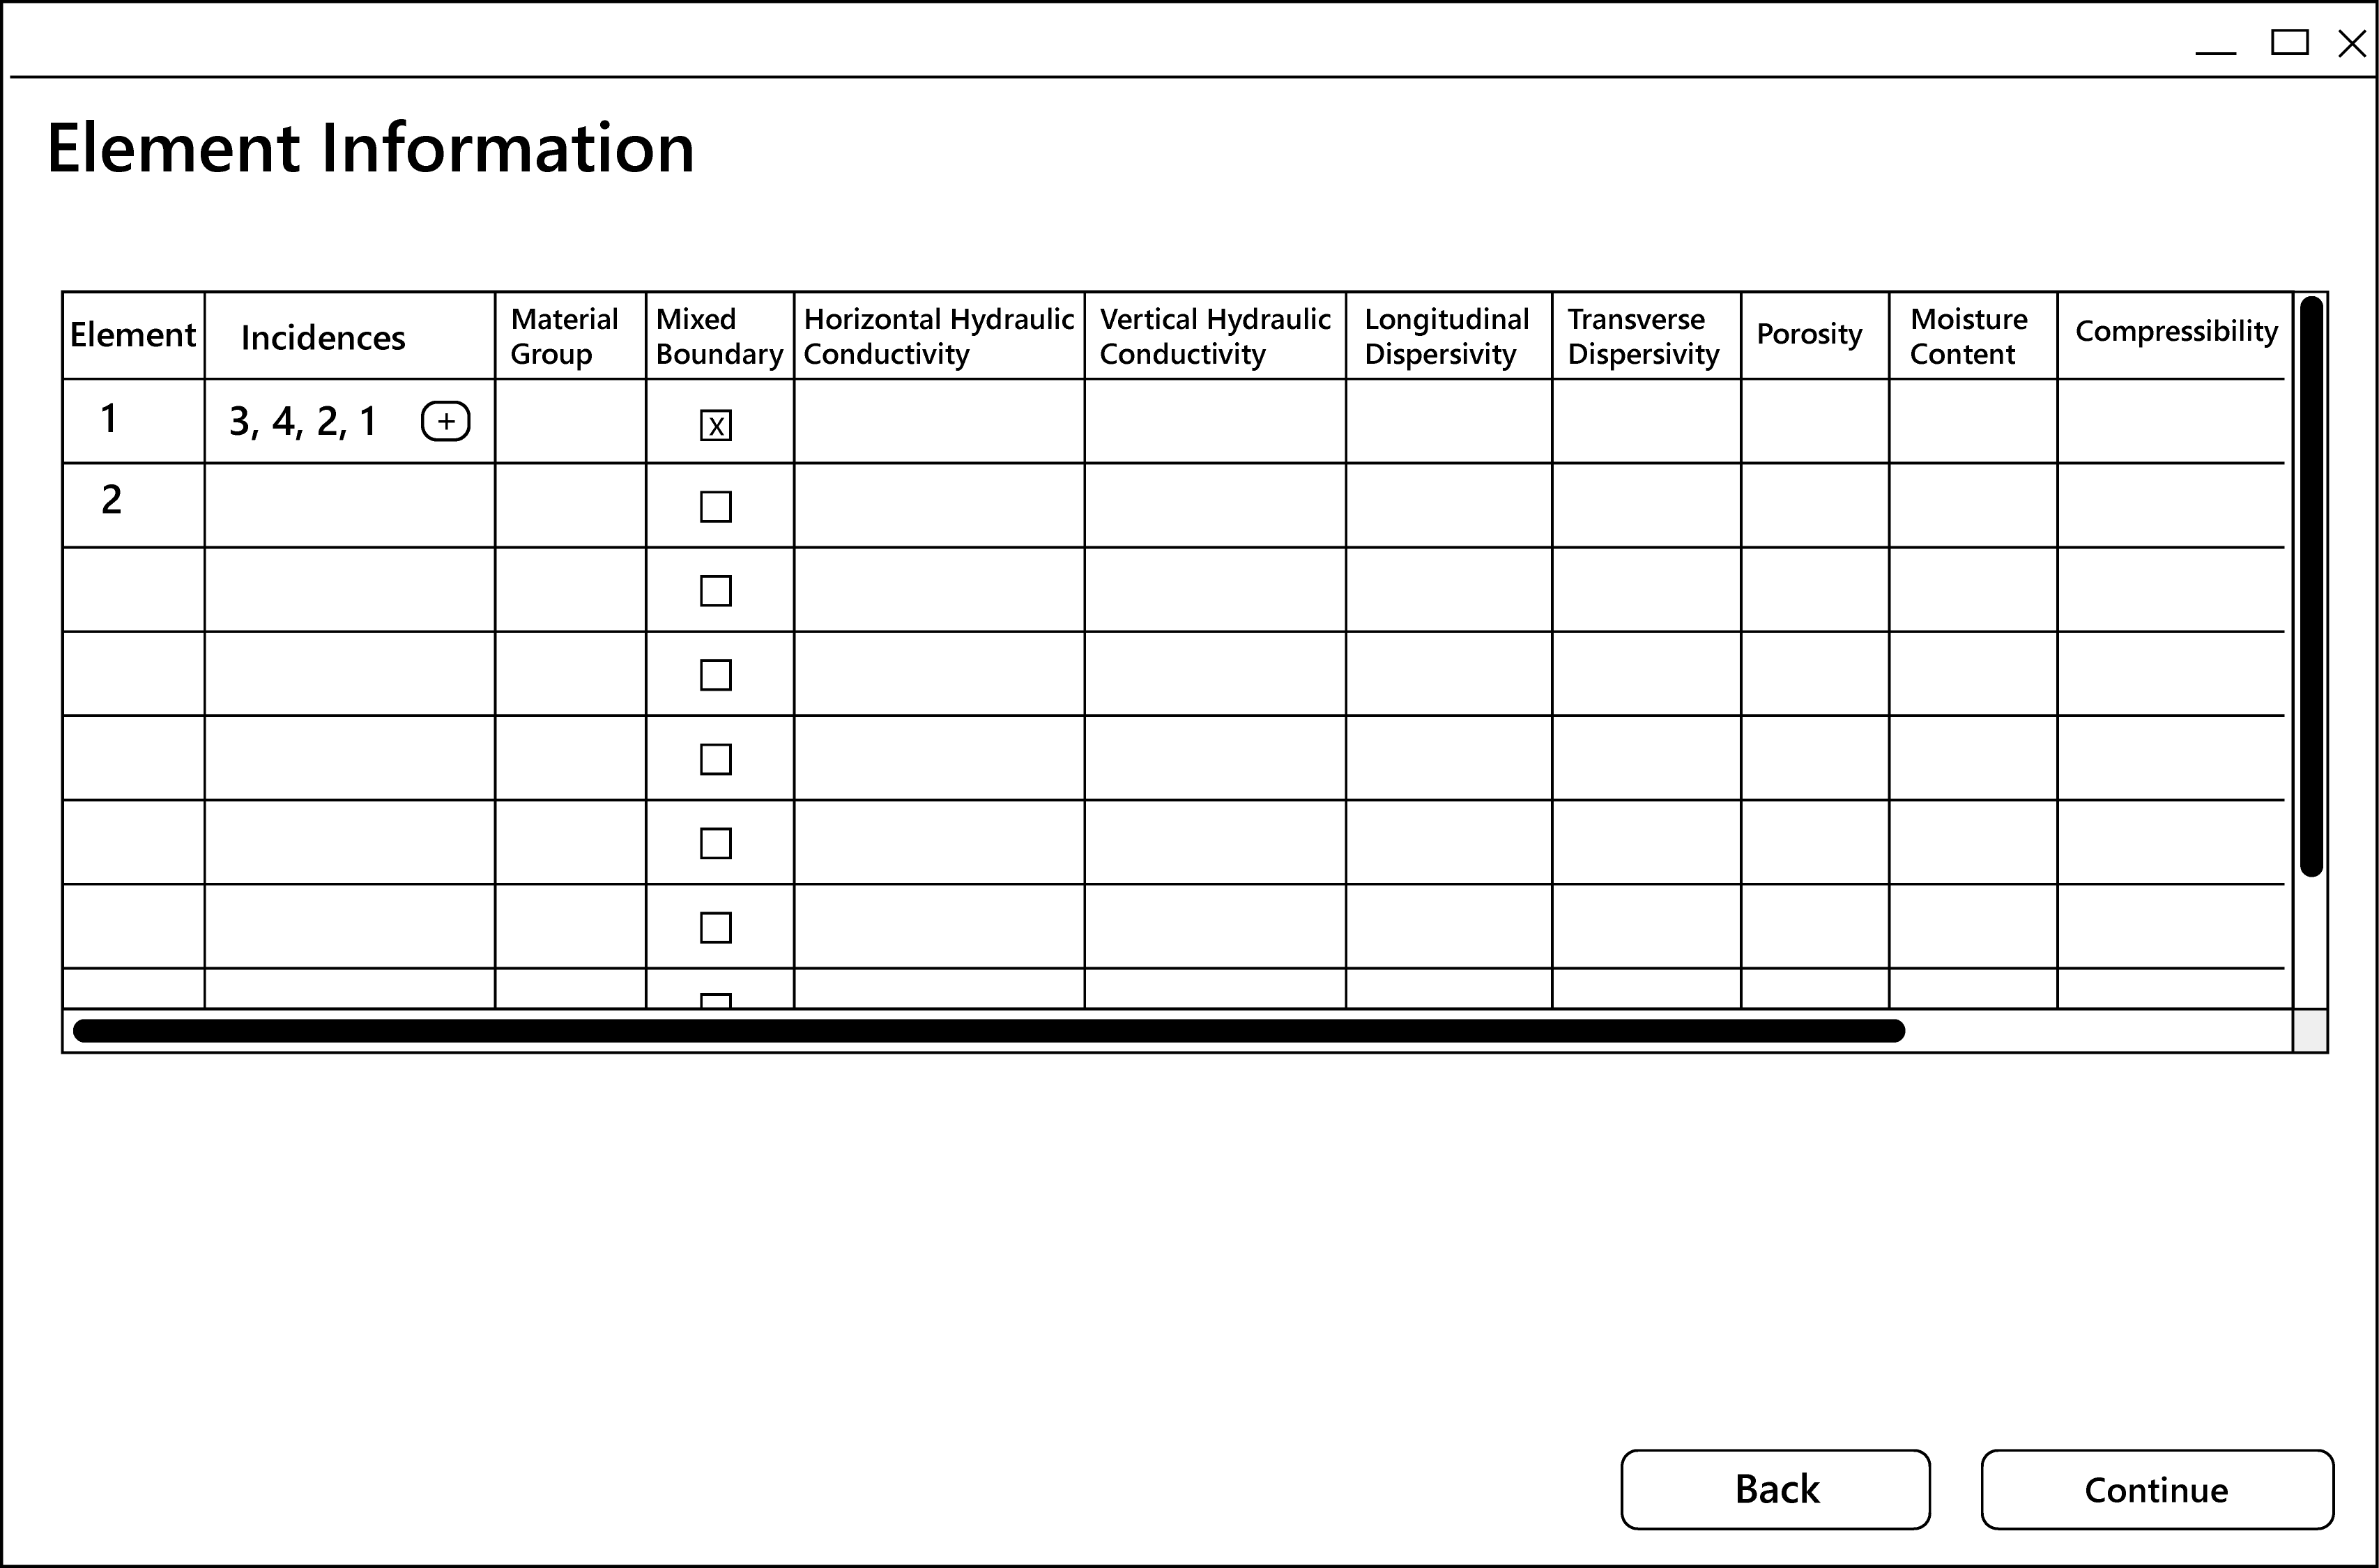
\includegraphics[scale=0.5]{GS2_element.png}
\caption{Screen to set element data}
\label{fig:Element Information Screen}
\end{figure}

\begin{figure}[H]
\centering
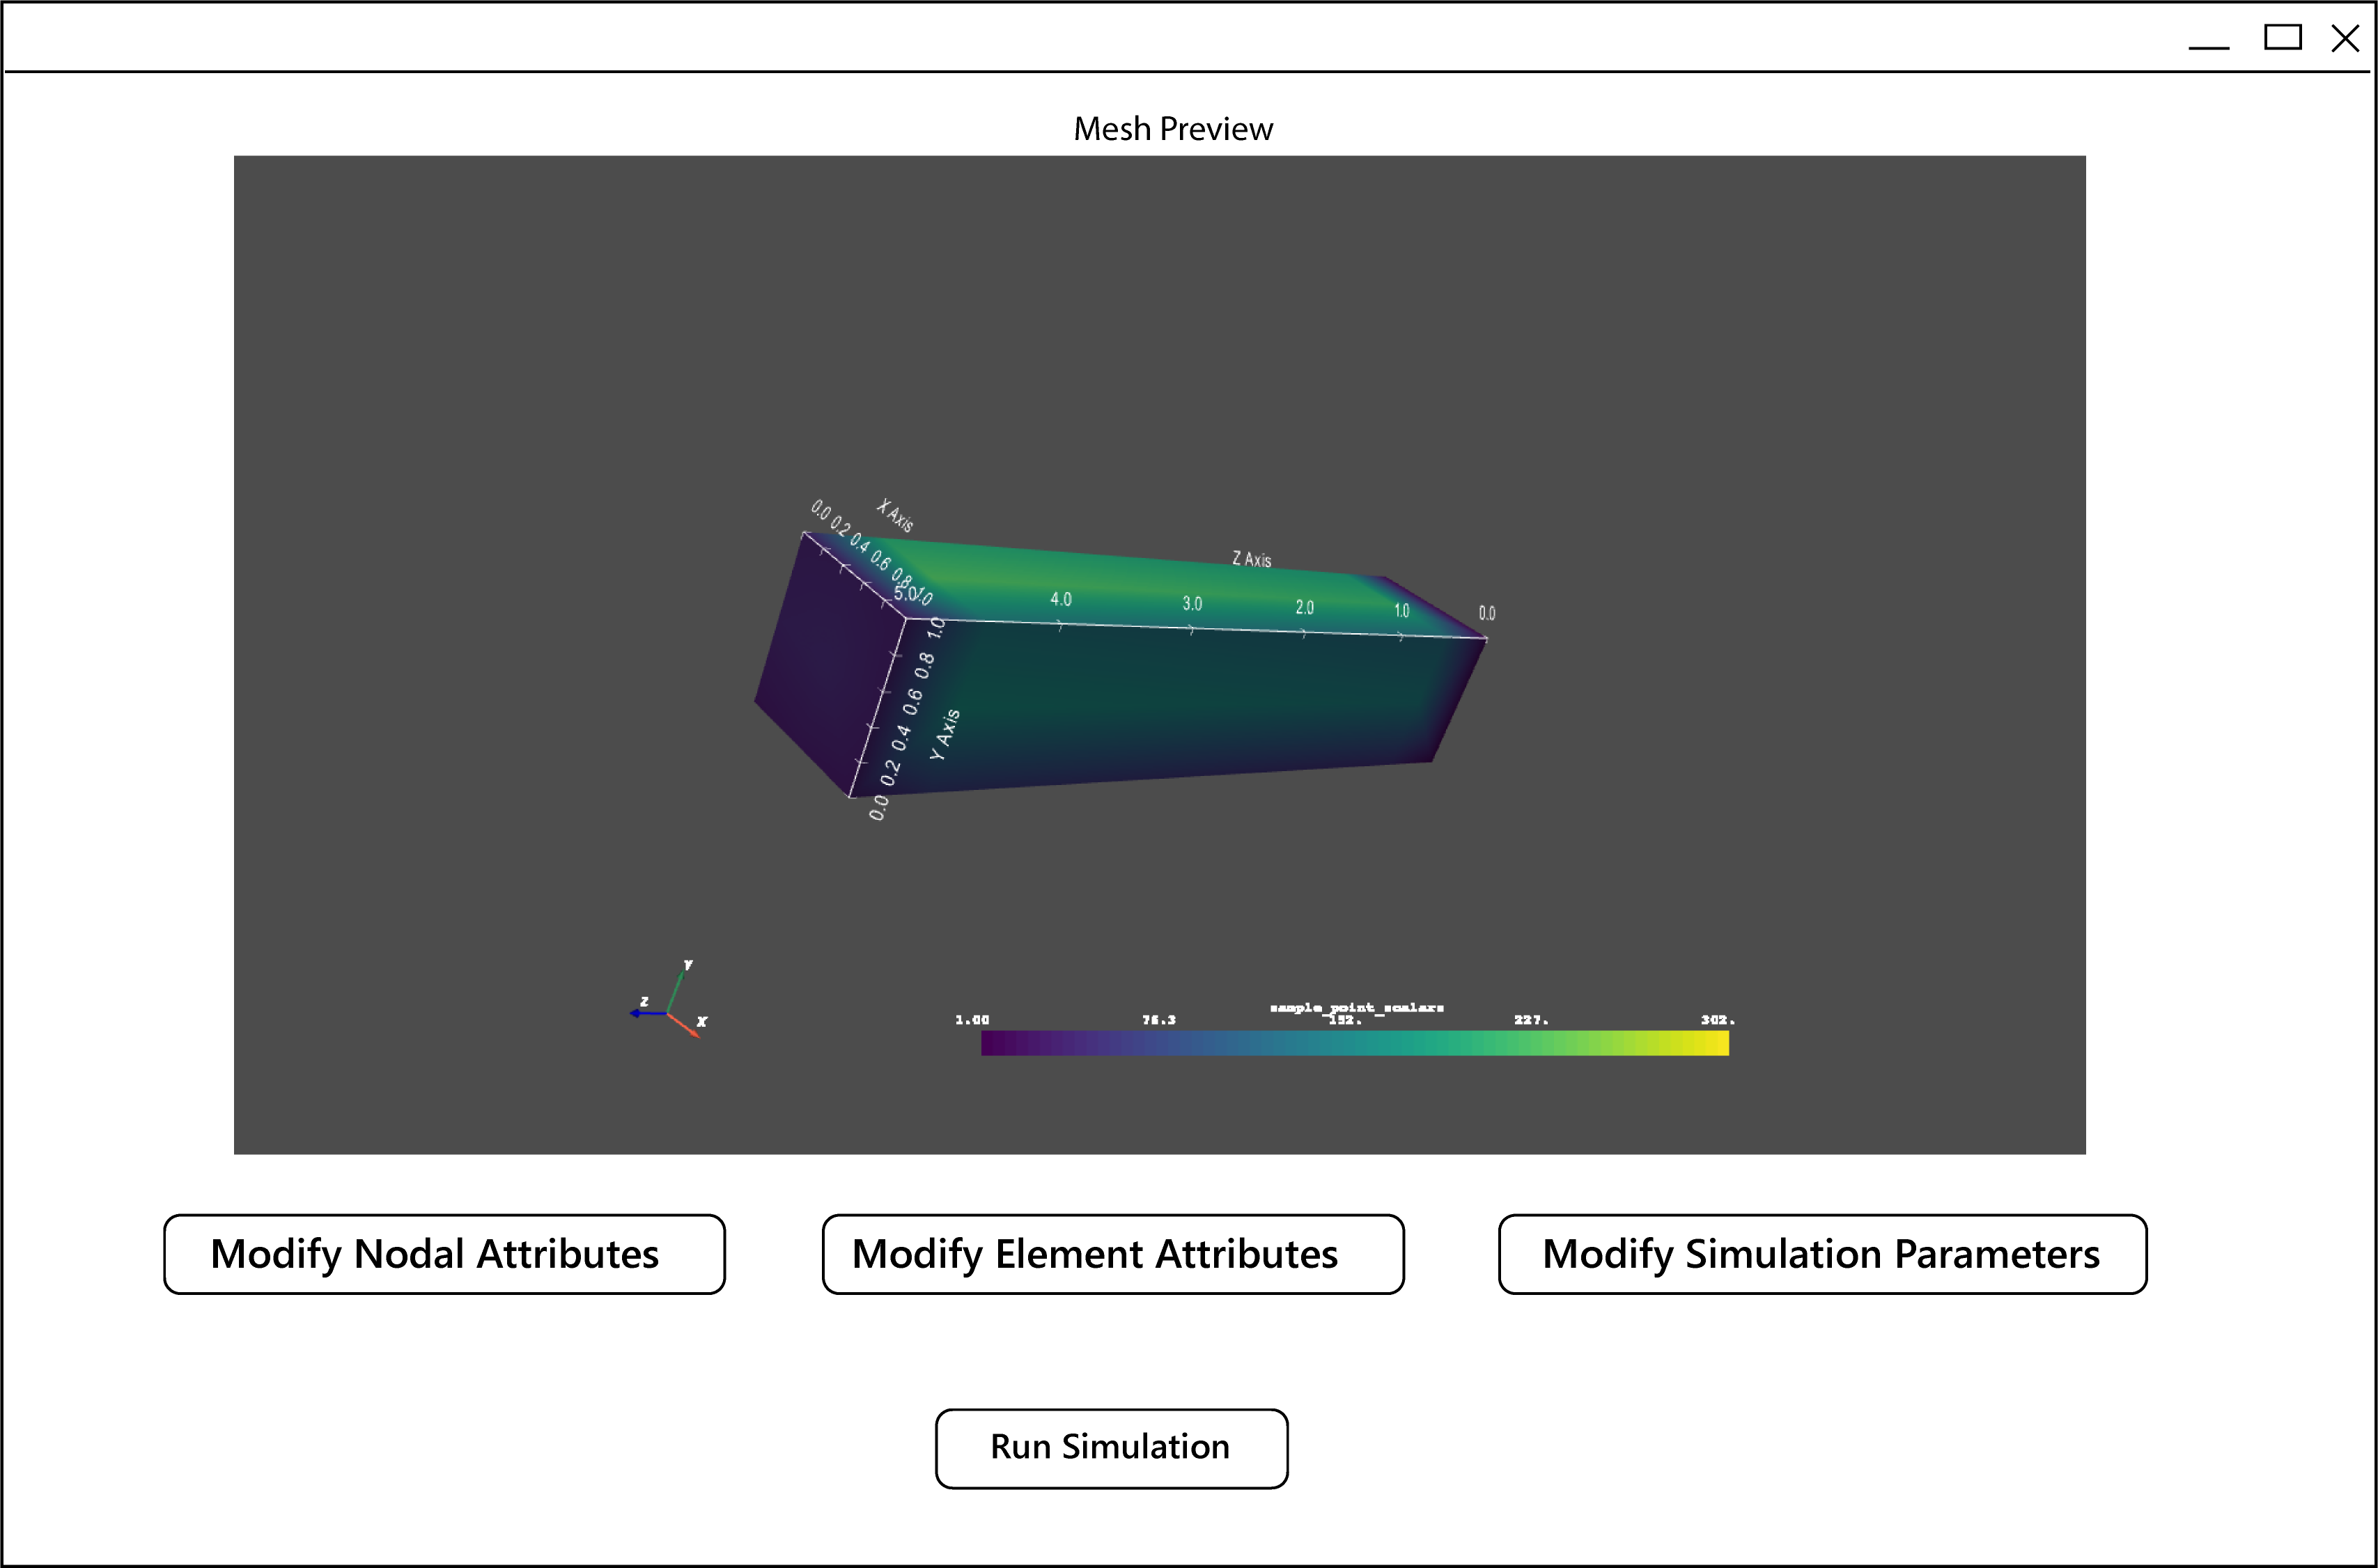
\includegraphics[scale=0.5]{GS_preview.png}
\caption{Preview screen to show mesh and allow modifications}
\label{fig:Mesh Preview Screen}
\end{figure}

\subsubsection{Design Decisions}
The GUI provides numerous input fields for users to supply data specific to their mesh and the variables that influence this mesh. Because a mesh could contain hundreds if not thousands of individual nodes, a table was used to display information and allow users to modify that information. This decision was made to allow users to preview information for multiple nodes in a single window, and have the ability to modify the attributes that define these nodes. This same reasoning was used for the window containing element information. The GUI provides a sequential order for supplying data specific to each simulation: simulation parameters, nodal information, and element information but users will be able to transition between sections as they see fit.

\subsection{CLI}
\subsubsection{Context}
A command-line interface will also be available for users wanting to bypass the GUI and still be able to execute a simulation. This will require the user to include two file names when executing the main program. This can be done via a command prompt with the command:
\begin{lstlisting}[language=bash]
  $ python3 main_prog.py -in nodal_information.txt -out sim_results.txt
\end{lstlisting}

Order does not matter, as long as the command is immediately followed by the file path. The command '-in' is followed by the path to an input file containing all appropriate parameters for each node included in the model. The command '-out' is followed by the name of the file used to save the results of the simulation.

\end{document}
